\section{Numerical validation of eq.~\eqref{eq:EpsilonZeroMode}}
\label{app:zero_mode}
In eq.~\eqref{eq:EpsilonZeroMode} we showed that the solution for
$\varepsilon_{\infty}$ in the limit of infinite training length corresponds to
the zero mode of the evolution matrix in data space $\tilde{H}_{\varepsilon}$.
Here we provide the numerical argument that supports this result.

We start from the matrix $M$ which, roughly speaking, is the contraction of two
FK tables. Since FK tables contain many zeros, the matrix $M$ will be sparse.
The matrix $M$ is displayed element-wise in Fig.~\ref{fig:MatrixM}. Each block
identifies a flavour, and the length of the side of the block is equal to the
size of the grid. 
% Figure ----------------------
\begin{figure}[h]
  \centering
  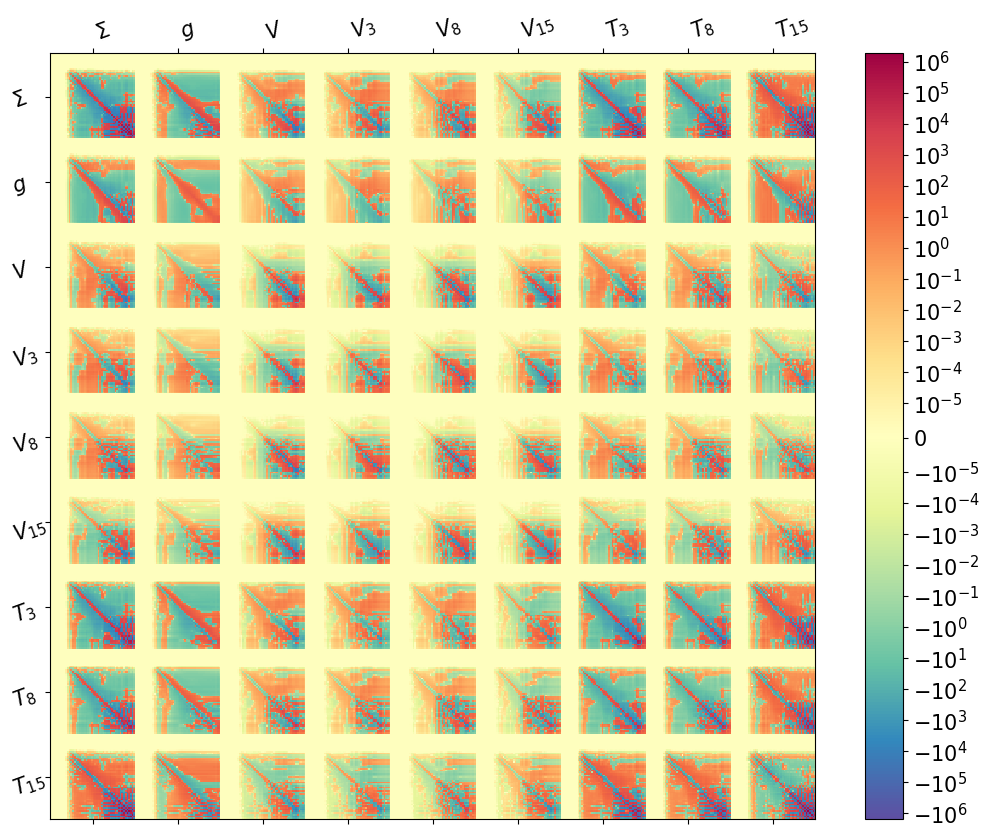
\includegraphics[width=0.5\textwidth]{M_matrix.png}
  \caption{\small Matrix $M$ in logarithmic scale.}
  \label{fig:MatrixM}
\end{figure}
%----------------------
The matrix $M$ is decomposed using the singular value decomposition (SVD) method
\begin{equation}
M = U \Sigma V^T \,,
\end{equation}
where $U$ and $V$ are orthogonal matrices, and $\Sigma$ is a diagonal matrix
containing the singular values sorted in decreasing order. Recall that the
matrix $M$ is also symmetric by construction, and this guarantees the existence
of the solution of the associated eigensystem. Singular values and the absolute
eigenvalues are displayed in Fig.~\ref{fig:eig_svd_M}. Here we also show the
relative machine precision error, defined as the product of the largest singular
value with the machine precision for double precision floating numbers
($\epsilon \sim 2.2 \times 10^{-16}$). Since the largest singular value is of
order $10^6$, the relative machine precision error is
$\epsilon_{\textrm{rel}}\sim1.2\times 10^{-9}$. The relevance of this number
will be clear in the following observation.

As it can be seen from the figure, the singular values and the eigenvalues
overlap as long as the relative numerical precision is not reached. Once this
numerical threshold is exceeded, the two sets of values start to diverge. This
is a consequence of the fact that $\epsilon_{\textrm{rel}}$ defines the smallest
double floating number that machine precision allows us to distinguish.
Everything below this value is noise and should be discarded. This prompts us to
apply an \textit{ad hoc} regularisation to $\Sigma$, whereby the values below
$\epsilon_{\textrm{rel}}$ are set to zero.
% Figure ----------------------
\begin{figure}[h]
  \centering
  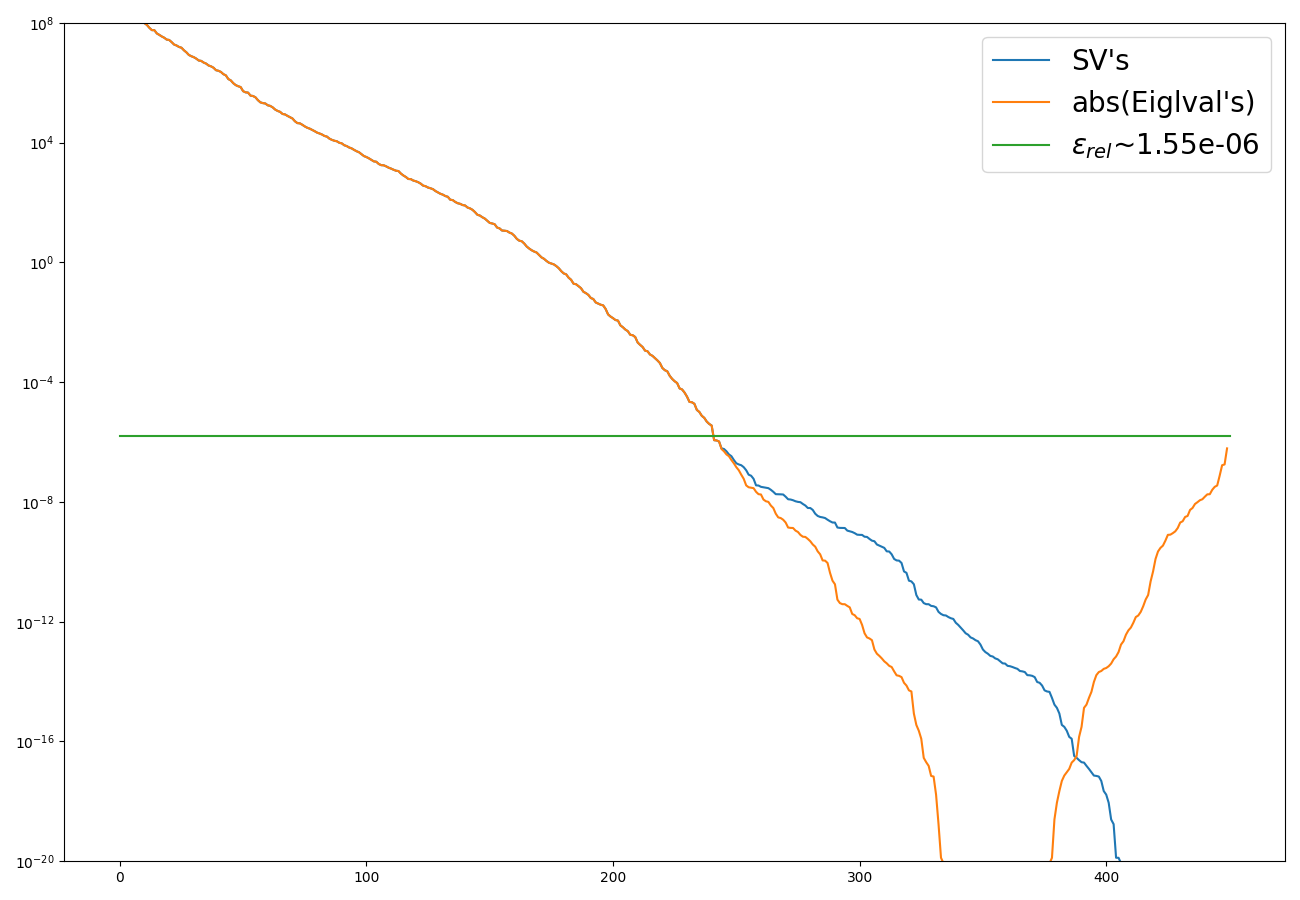
\includegraphics[width=0.5\textwidth]{eig_svd_M.png}
  \caption{\small Singular values and (absolute) eigenvalues of the matrix $M$
    plotted in logarithmic scale. The green horizontal line marks the relative
    machine precision error, as explained in the main text.}
  \label{fig:eig_svd_M}
\end{figure}
%----------------------
Note that we have also checked that the singular vectors of $U$ and $V$ are the
same if they are associated to the singular values above the numerical
threshold. In other words, in the space orthogonal to Ker$(M)$, the SVD matches
the eigendecomposition.

In principle, the singular vectors of the non-zero values span the space
orthogonal to Ker$(M)$. In this subspace, the matrix $M$ is diagonal and the
entries are exactly the non-zero singular values. However, if we compute the
condition number of $M$ in this subspace, we find that it is remarkably large,
$\kappa(M) \sim 10^{15}$. In other words, even in this subspace the matrix $M$
is ill-defined and cannot be inverted. The solution to this problem is to
further reduce the dimensionality of the orthogonal space, at the cost of
introducing some arbitrariness into the problem. Specifically, the final
solution will depend on the number of small singular values that we discard. For
example, the solution at infinity, eq.~\eqref{eq:InfiniteTrainingF}, will be
influenced by this cut-off, as shown in Fig.~\ref{fig:InfiniteTrainingFCuts}. In
this figure, eq.~\eqref{eq:InfiniteTrainingF} is first computed in the truncated
orthogonal space; then the result is transformed back to the original flavour
basis using the matrix $U$ restricted to the vectors that span the (reduced)
orthogonal space.
% Figure ----------------------
\begin{figure}[h]
  \centering
  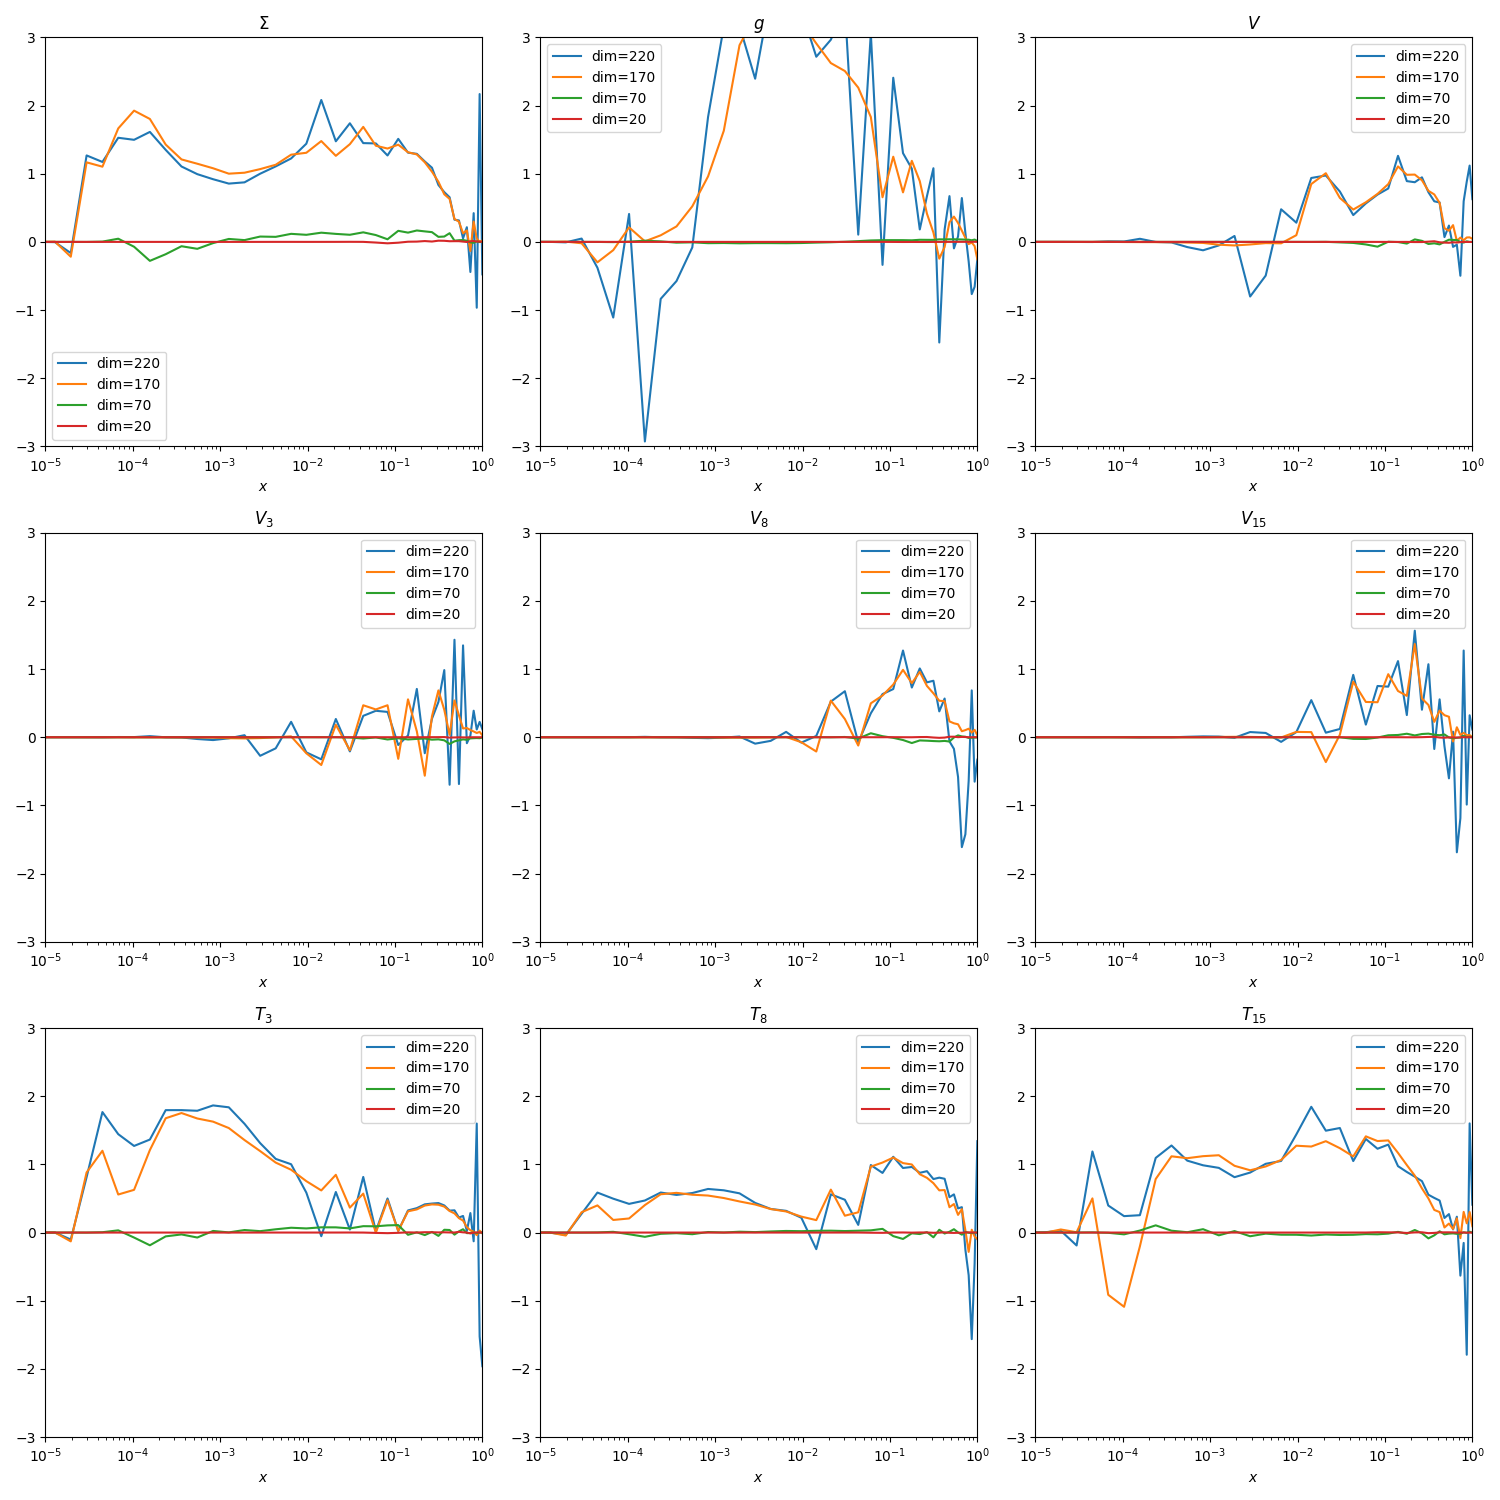
\includegraphics[width=0.7\textwidth]{f_inf.png}
  \caption{\small}
  \label{fig:InfiniteTrainingFCuts}
\end{figure}
%----------------------

As a final check, we can verify that eq.~\eqref{eq:EpsilonZeroMode} is
numerically satisfied. As we have just mentioned, even $\epsilon_{\infty}$ will depend
on the severity of the cut-off. We then expect different results as we modify the
number of singular values that we discard. For instance, using the orthogonal
subspace without any cut, eq.~\eqref{eq:EpsilonZeroMode} evaluates to
\begin{equation}
  \left| \tilde{H}_{\varepsilon} \varepsilon_{\infty} \right| \approx 0.28 \,.
\end{equation}
On the other hand, if we reduce the size of the subspace to $170$ (from 320), we
get
\begin{equation}
  \left| \tilde{H}_{\varepsilon} \varepsilon_{\infty} \right| \approx ~1.33 \times 10^{-5} \,.
\end{equation}

